\documentclass[12pt,a4paper]{article}

\usepackage[utf8]{inputenc}
\usepackage[margin=1in]{geometry}
\usepackage{amsmath, amssymb}
\usepackage{graphicx}
\usepackage{booktabs}
\usepackage{hyperref}
\usepackage{caption}
\usepackage{subcaption}
\usepackage{cite}

\hypersetup{colorlinks=true, linkcolor=blue, citecolor=red, urlcolor=blue}

% numbers produced by `python main.py orr-sommerfeld`
% auto-generated by main.py orr-sommerfeld
\newcommand{\osYinf}{8}
\newcommand{\osNsteps}{1500}
\newcommand{\osNRe}{41}
\newcommand{\osNAlpha}{41}
\newcommand{\osReMin}{200}
\newcommand{\osReMax}{20000}
\newcommand{\osAlphaMin}{0.02}
\newcommand{\osAlphaMax}{0.42}
\newcommand{\osRec}{519.06}
\newcommand{\osAlphac}{0.3037}
\newcommand{\osCrc}{0.3966}
\newcommand{\osRuntime}{111}


\title{\textbf{Linear Stability of the Blasius Boundary Layer:\\ Base-Flow Computation, Orr--Sommerfeld Shooting and the Neutral Curve} \\[0.5em]
\large Assignment --- ME/AE Numerical Methods}
\author{Harikesh \\ Roll No: 24JE0271}
\date{\today}

\begin{document}

\maketitle

\begin{abstract}
This report computes the neutral stability curve of the flat-plate (Blasius) boundary layer from the Orr--Sommerfeld equation under the parallel-flow approximation. The base flow is first obtained from the Blasius equation $f''' + \tfrac12 ff'' = 0$ with three independent methods: collocation (\texttt{solve\_bvp}), shooting with \texttt{solve\_ivp}, and a from-scratch RK4 shooting method. All three give $f''(0) = 0.33205734$ and $\delta^* = 1.7208$. Using this profile, the Orr--Sommerfeld equation is solved by shooting. The two disturbance solutions that decay in the freestream are started at $y_\infty = \osYinf\,\delta^*$ and integrated down to the wall with RK4 in compound-matrix form, which removes the parasitic growth that otherwise makes the two solutions numerically dependent. Imposing no-slip at the wall gives a dispersion relation $D(\alpha, Re, c) = 0$, which is solved for the complex wave speed $c$ by Newton--Raphson. The solver reproduces Jordinson's benchmark eigenvalue to $10^{-7}$. A sweep over \osNAlpha$\times$\osNRe{} values of $(\alpha, Re)$ maps the growth rate $c_i$, and the refined neutral curve $c_i = 0$ gives a critical Reynolds number $Re_{\delta^*,c} = \osRec$ at $\alpha_c\delta^* = \osAlphac$ with phase speed $c_r = \osCrc$, in agreement with the classical value $Re_{\delta^*,c} \approx 520$.
\end{abstract}

\tableofcontents
\newpage

% ================================================================
\section{Introduction}
% ================================================================

A laminar boundary layer on a flat plate stays laminar only up to a point. Beyond a certain Reynolds number, small disturbances in the form of two-dimensional travelling waves (Tollmien--Schlichting, or TS, waves) are amplified, and their growth is the first stage of the classical route to transition. Linear stability theory predicts where this amplification begins. For each Reynolds number it gives the band of wavenumbers that grow, and the boundary of that band in the $(Re, \alpha)$ plane is the \emph{neutral curve}. Its leftmost point, the \emph{critical Reynolds number}, is the lowest Reynolds number at which any infinitesimal disturbance can grow.

The analysis has two parts:
\begin{enumerate}
    \item \textbf{Base flow} (Section~\ref{sec:blasius}). The Blasius similarity equation is solved accurately with three methods, which cross-check one another. The result is rescaled to displacement-thickness units.
    \item \textbf{Stability} (Sections~\ref{sec:os}--\ref{sec:results}). The Orr--Sommerfeld eigenvalue problem is solved by shooting from the freestream to the wall at many $(Re, \alpha)$, and the neutral curve and critical point are extracted.
\end{enumerate}
Both stages run with a single command, \texttt{python main.py orr-sommerfeld}, which always computes the Blasius base flow first.

% ================================================================
\section{Base Flow: The Blasius Boundary Layer}
\label{sec:blasius}
% ================================================================

\subsection{Similarity equation}

For steady flow over a semi-infinite flat plate at zero incidence, the similarity variables $\eta = y\sqrt{U_\infty/\nu x}$ and $\psi = \sqrt{\nu x U_\infty}\, f(\eta)$ reduce the boundary layer equations to~\cite{blasius1908}
\begin{equation}
    f''' + \tfrac{1}{2} f f'' = 0, \qquad f(0) = 0,\quad f'(0) = 0,\quad f'(\infty) = 1,
    \label{eq:blasius}
\end{equation}
with $u/U_\infty = f'(\eta)$. The quantities of interest are the wall shear $f''(0)$, which gives $C_f = 0.664/\sqrt{Re_x}$, and the displacement thickness
\begin{equation}
    \frac{\delta^*}{\sqrt{\nu x / U_\infty}} = \int_0^\infty (1 - f')\, d\eta = \lim_{\eta\to\infty}(\eta - f) = 1.7208,
\end{equation}
which sets the length scale of the stability problem.

\subsection{Three solution methods}

With $\mathbf{y} = [f, f', f'']^T$, Equation~\eqref{eq:blasius} becomes a first-order system with $y_2' = -\tfrac12 y_0 y_2$. The far-field condition is applied at $\eta_\infty = 10$.
\begin{itemize}
    \item \textbf{Collocation} (\texttt{scipy.integrate.solve\_bvp}): a 4th-order Lobatto~IIIA scheme with adaptive mesh refinement, started from the guess $f' \approx \tanh(\eta/2)$.
    \item \textbf{Shooting with \texttt{solve\_ivp}}: the unknown $s = f''(0)$ is adjusted by Newton--Raphson until $\Phi(s) = f'(\eta_\infty; s) - 1 = 0$, with $\Phi'(s)$ from a forward finite difference ($\varepsilon = 10^{-6}$).
    \item \textbf{Scratch RK4 shooting}: a fixed-step RK4 integrator ($h = 0.01$) advances $\mathbf{y}$ together with the sensitivities $\mathbf{z} = \partial\mathbf{y}/\partial s$, which satisfy $z_2' = -\tfrac12(z_0 f'' + f z_2)$ with $\mathbf{z}(0) = [0, 0, 1]^T$. This gives the exact Newton derivative $\Phi'(s) = z_1(\eta_\infty)$ from a single integration per iteration.
\end{itemize}

\subsection{Results}

\begin{table}[htbp]
  \centering
  \caption{Blasius base flow: comparison of the three methods ($\eta_\infty = 10$). Benchmark $f''(0) = 0.3320573362$.}
  \label{tab:blasius}
  \begin{tabular}{lcccccc}
    \toprule
    Method & $f''(0)$ & Error & $\delta_{99}$ & $\delta^*$ & $\theta$ & $H$ \\
    \midrule
    \texttt{solve\_bvp} & 0.3320573372 & 1.01e-09 & 4.9101 & 1.7208 & 0.6641 & 2.5912 \\
    \texttt{solve\_ivp} + Newton & 0.3320573372 & 9.81e-10 & 4.9100 & 1.7208 & 0.6641 & 2.5912 \\
    Scratch RK4 + Newton & 0.3320573372 & 9.90e-10 & 4.9100 & 1.7208 & 0.6641 & 2.5911 \\
    \midrule
    Literature & 0.3320573362 & --- & 4.91 & 1.7208 & 0.6641 & 2.5911 \\
    \bottomrule
  \end{tabular}
\end{table}


Table~\ref{tab:blasius} shows that the three methods agree with one another to a few times $10^{-11}$, and with the benchmark $f''(0) = 0.332057336$ to about $10^{-9}$. The integral thicknesses match the classical values~\cite{schlichting2016, white2006}. Both shooting methods converge quadratically in four Newton iterations (Figure~\ref{fig:bl_conv}). The truncation study shows that the error in $f''(0)$ falls from $2\times10^{-2}$ at $\eta_\infty = 4$ to $10^{-9}$ at $\eta_\infty = 10$, consistent with $1 - f' \sim e^{-\eta^2/4}$. The RK4 order-of-accuracy check is in Appendix~\ref{app:blasius}.

\begin{figure}[h]
    \centering
    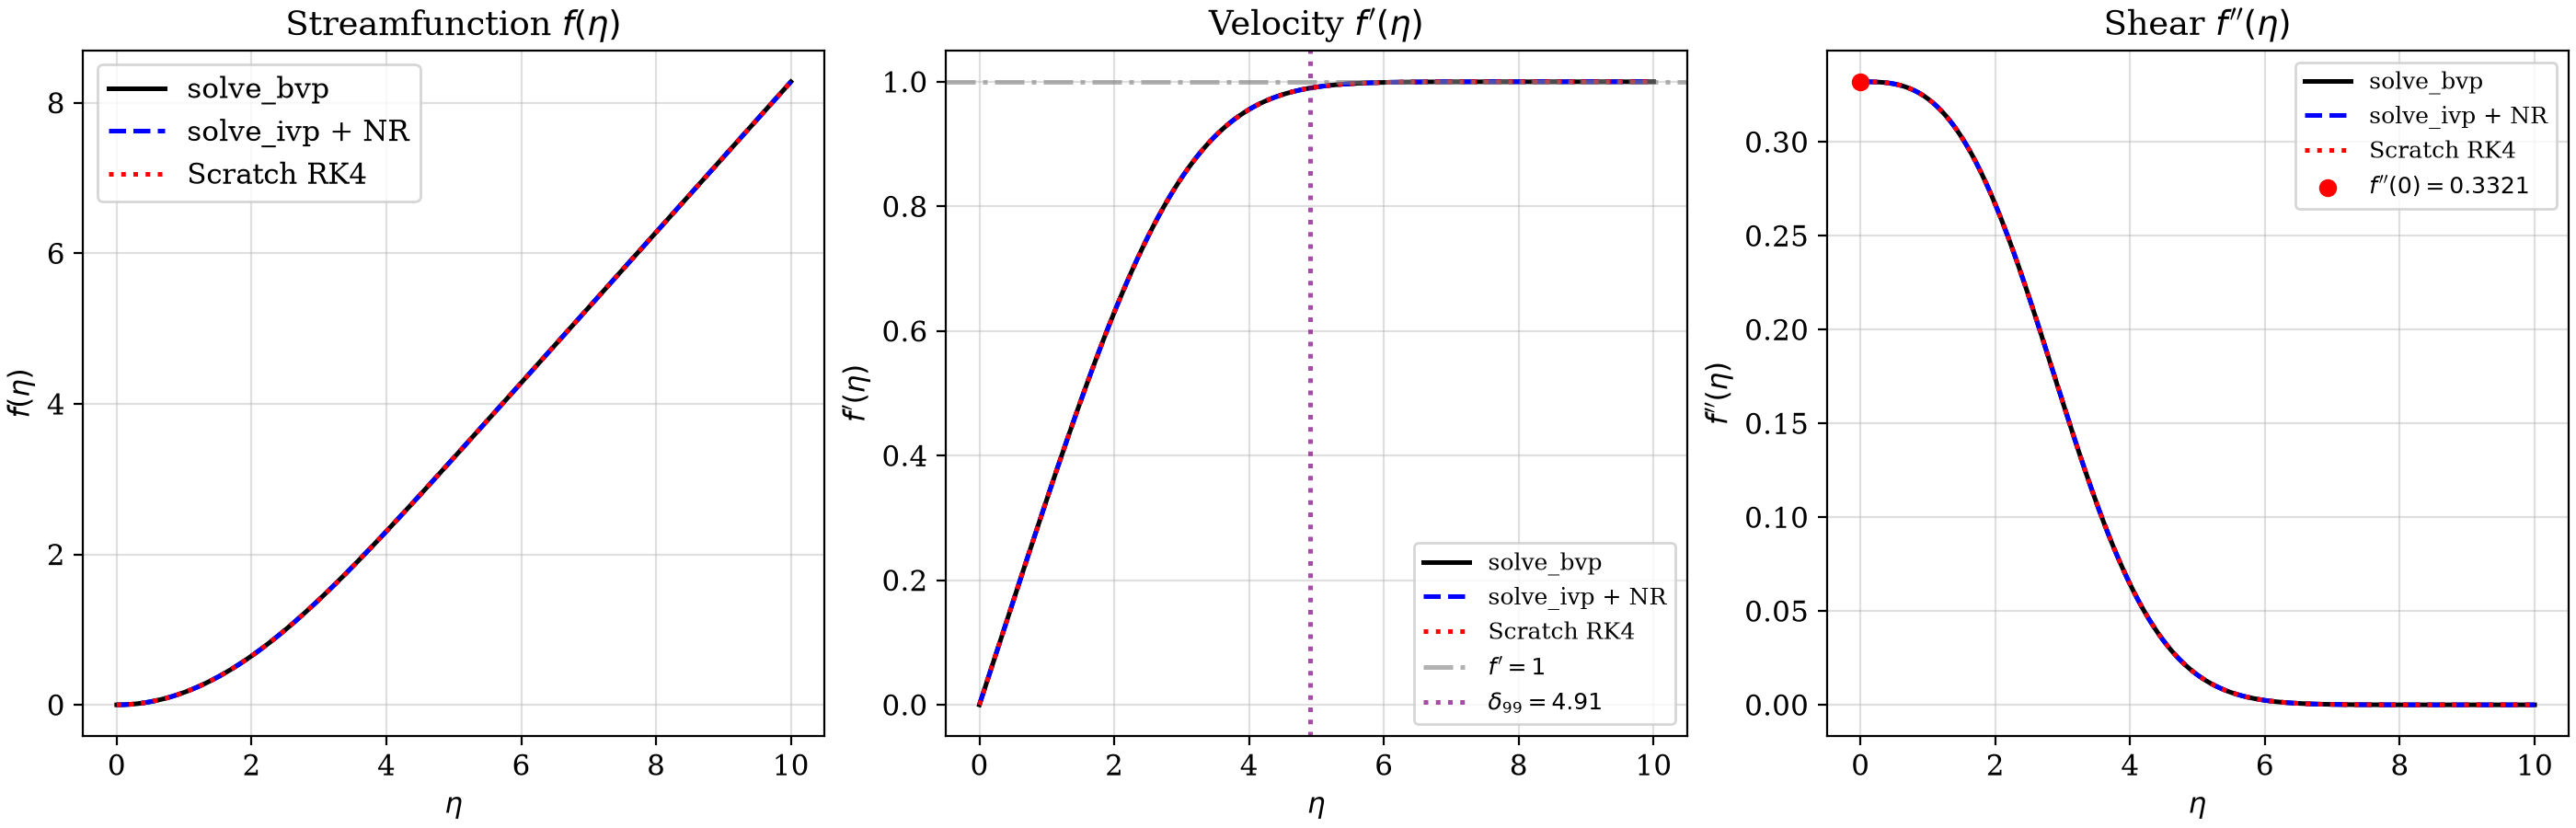
\includegraphics[width=\textwidth]{figures/blasius_profiles.png}
    \caption{Blasius solution $f$, $f'$, $f''$ from the three methods. The curves are indistinguishable at plotting scale.}
    \label{fig:bl_prof}
\end{figure}

\begin{figure}[h]
    \centering
    \begin{subfigure}[b]{0.48\textwidth}
        \centering
        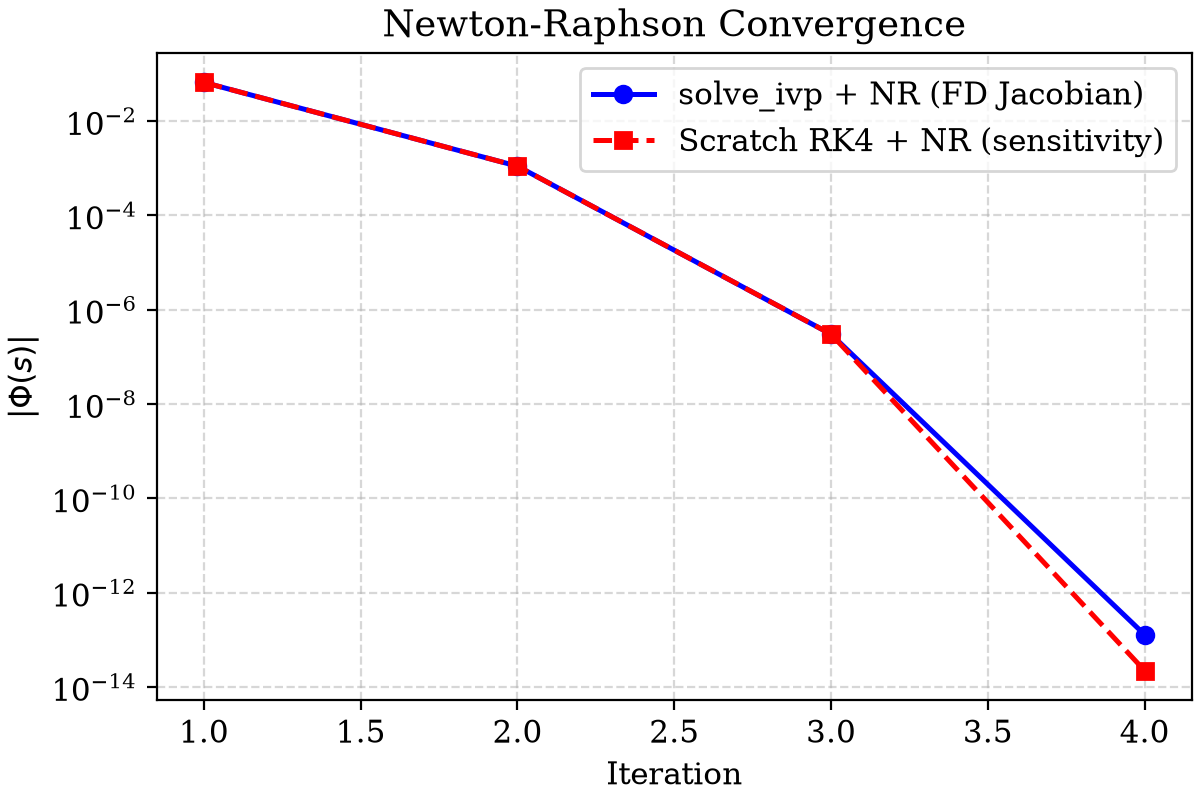
\includegraphics[width=\textwidth]{figures/blasius_newton_convergence.png}
        \caption{Newton--Raphson residual history.}
    \end{subfigure}
    \hfill
    \begin{subfigure}[b]{0.48\textwidth}
        \centering
        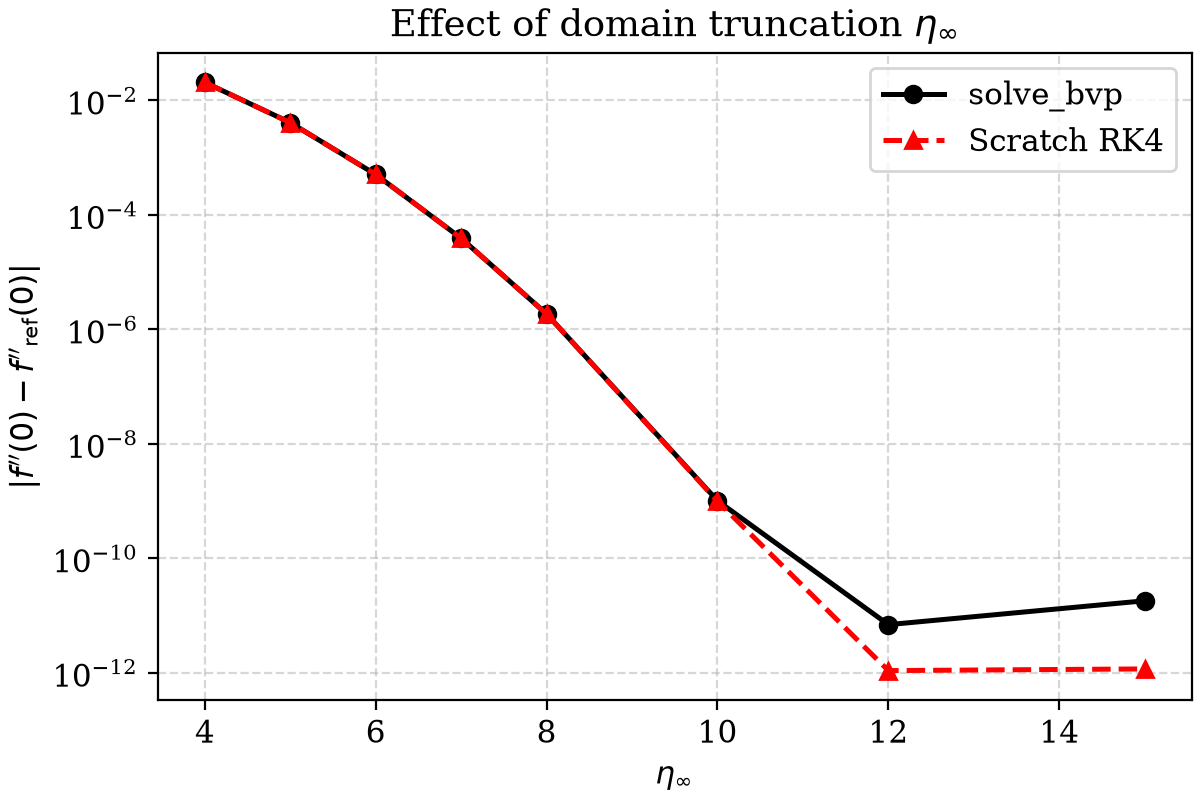
\includegraphics[width=\textwidth]{figures/blasius_eta_inf_study.png}
        \caption{Error in $f''(0)$ against $\eta_\infty$.}
    \end{subfigure}
    \caption{Convergence of the Blasius shooting solvers.}
    \label{fig:bl_conv}
\end{figure}

\subsection{Base flow for the stability analysis}

For the stability problem, lengths are scaled with $\delta^*$ and velocities with $U_\infty$:
\begin{equation}
    y = \frac{\eta}{1.72079}, \qquad Re \equiv Re_{\delta^*} = \frac{U_\infty\delta^*}{\nu} = 1.72079\sqrt{Re_x}, \qquad
    U(y) = f'(\eta), \qquad U''(y) = -\tfrac12 f f''\,(1.72079)^2 .
\end{equation}
The Orr--Sommerfeld solver needs $U$ and $U''$ at arbitrary $y$, so $f''(0)$ is taken from the collocation solution and the profile is re-integrated from the wall with a tight-tolerance DOP853 integrator ($\text{rtol} = 10^{-12}$) using dense output. Figure~\ref{fig:base} shows the result. $U''$ is negative everywhere and vanishes at the wall, so the profile has no inflection point. By Rayleigh's criterion it is therefore inviscidly stable, and any instability must come from viscosity: these are the TS waves.

\begin{figure}[h]
    \centering
    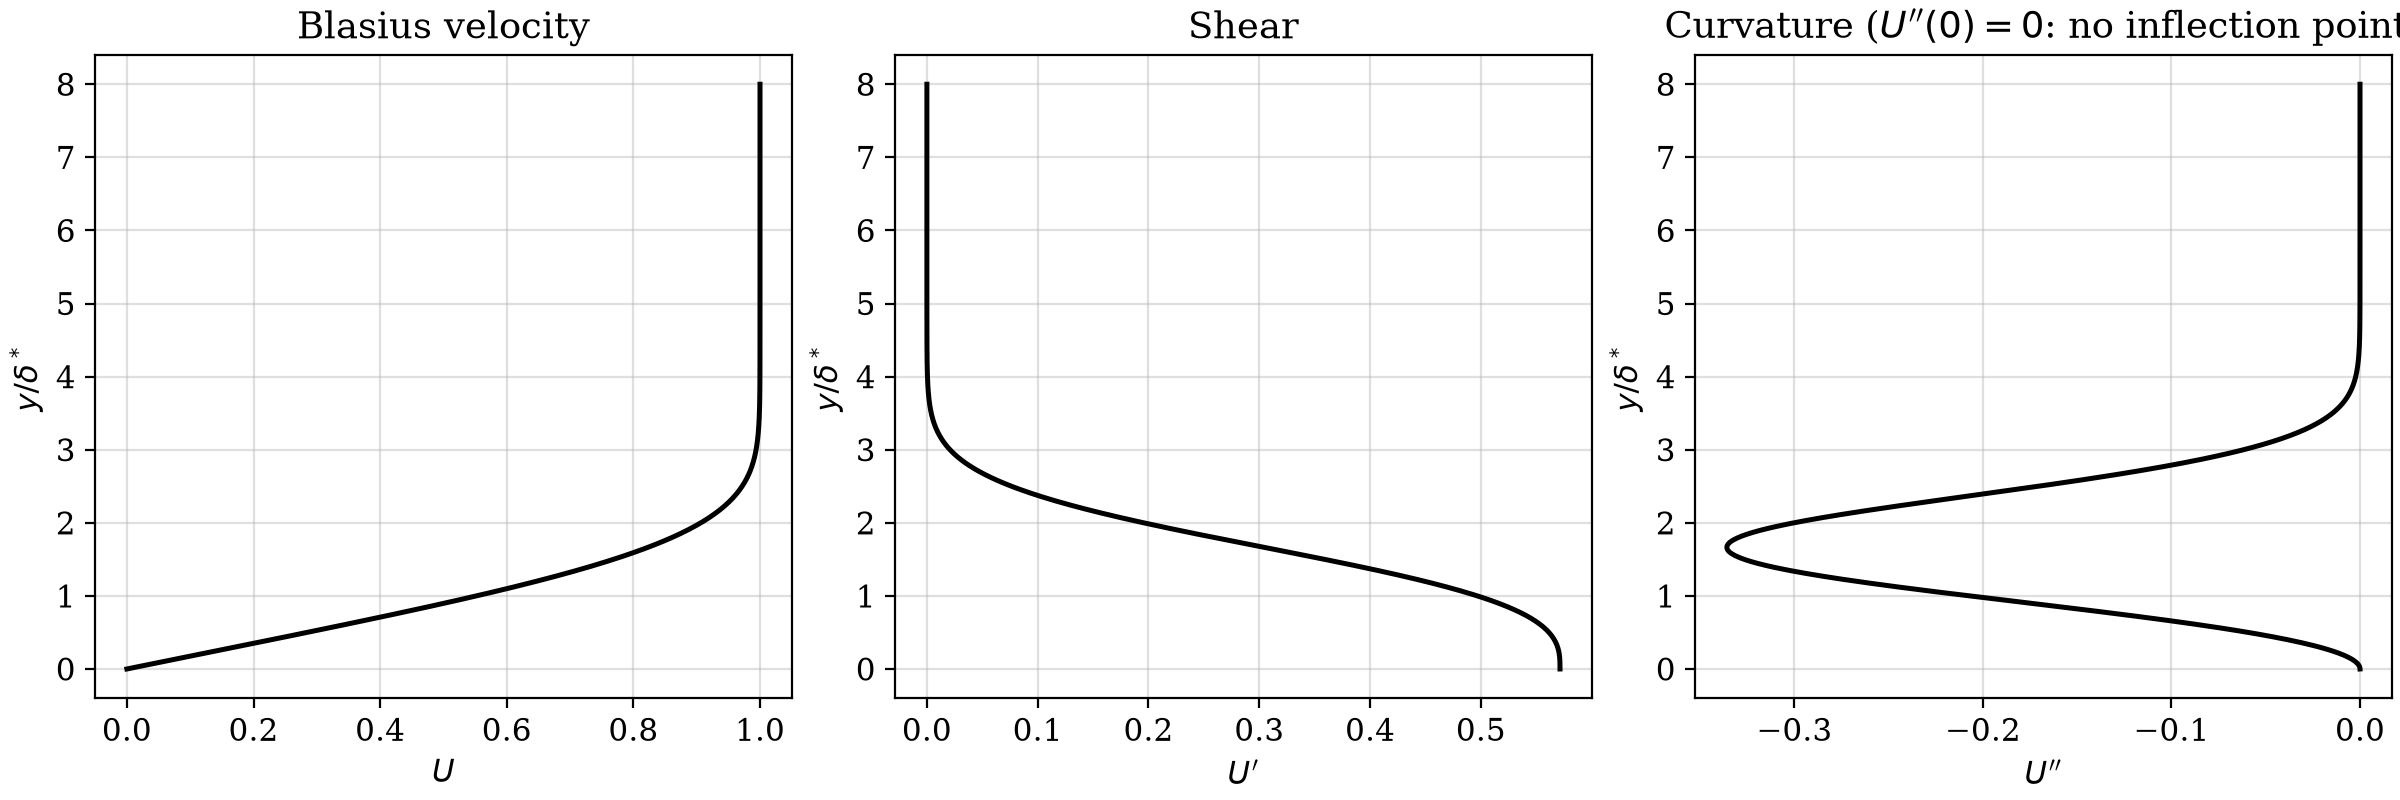
\includegraphics[width=\textwidth]{figures/base_flow.png}
    \caption{Blasius base flow in displacement-thickness units, as used in the Orr--Sommerfeld equation.}
    \label{fig:base}
\end{figure}

% ================================================================
\section{The Orr--Sommerfeld Equation}
\label{sec:os}
% ================================================================

\subsection{Derivation under the parallel-flow approximation}

The boundary layer thickens slowly, like $\sqrt{x}$. Over one disturbance wavelength the base flow can therefore be treated as locally parallel, $\mathbf{U} = (U(y), 0)$, with $U$ evaluated at the local station: this is the \emph{parallel-flow approximation}. Linearising the incompressible Navier--Stokes equations about this flow and writing the two-dimensional disturbance through a streamfunction in normal-mode form,
\begin{equation}
    \psi'(x, y, t) = \phi(y)\, e^{i\alpha(x - ct)}, \qquad u' = \psi'_y,\ v' = -\psi'_x,
\end{equation}
then eliminating the pressure perturbation, gives the Orr--Sommerfeld equation~\cite{orr1907, sommerfeld1908, drazin2004}
\begin{equation}
    (U - c)(\phi'' - \alpha^2\phi) - U''\phi = \frac{1}{i\alpha Re}\left(\phi'''' - 2\alpha^2\phi'' + \alpha^4\phi\right),
    \label{eq:os}
\end{equation}
with no-slip and decay conditions
\begin{equation}
    \phi(0) = \phi'(0) = 0, \qquad \phi,\ \phi' \to 0 \quad (y \to \infty).
    \label{eq:osbc}
\end{equation}
Squire's theorem guarantees that for every unstable three-dimensional disturbance there is an unstable two-dimensional one at a lower Reynolds number, so the two-dimensional problem gives the critical Reynolds number.

\subsection{Temporal eigenvalue problem}

In the temporal formulation the wavenumber $\alpha$ is real and the wave speed $c = c_r + i c_i$ is the complex eigenvalue. The disturbance amplitude varies as $e^{\alpha c_i t}$, so
\begin{equation}
    c_i > 0:\ \text{unstable}, \qquad c_i = 0:\ \text{neutral}, \qquad c_i < 0:\ \text{stable}.
\end{equation}
The neutral curve is the locus $c_i(\alpha, Re) = 0$. For computation, Equation~\eqref{eq:os} is written as
\begin{equation}
    \phi'''' = A(y)\,\phi'' + B(y)\,\phi, \qquad
    A = 2\alpha^2 + i\alpha Re\,(U - c), \qquad B = -\alpha^4 - i\alpha Re\left[\alpha^2(U - c) + U''\right].
    \label{eq:osAB}
\end{equation}

% ================================================================
\section{Numerical Method: Shooting from the Freestream to the Wall}
\label{sec:method}
% ================================================================

\subsection{Freestream starting solutions}

For $y \ge y_\infty$ the base flow is uniform ($U = 1$, $U'' = 0$), so Equation~\eqref{eq:osAB} has constant coefficients and solutions $e^{\lambda y}$ with
\begin{equation}
    (\lambda^2 - \alpha^2)(\lambda^2 - \gamma^2) = 0, \qquad \gamma^2 = \alpha^2 + i\alpha Re\,(1 - c), \quad \operatorname{Re}\gamma > 0 .
\end{equation}
The decay conditions~\eqref{eq:osbc} allow only
\begin{equation}
    \phi_1 = e^{-\alpha y}\ \text{(inviscid solution)}, \qquad \phi_2 = e^{-\gamma y}\ \text{(viscous solution)}.
\end{equation}
These are evaluated analytically at $y = y_\infty$ and used as initial conditions. The integration then runs \emph{downward} to the wall, so the freestream conditions are satisfied exactly. The general decaying solution is $\phi = C_1\phi_1 + C_2\phi_2$, and a non-trivial $(C_1, C_2)$ satisfying $\phi(0) = \phi'(0) = 0$ exists only if
\begin{equation}
    D(\alpha, Re, c) \equiv \phi_1(0)\,\phi_2'(0) - \phi_2(0)\,\phi_1'(0) = 0 ,
    \label{eq:disp}
\end{equation}
which is the dispersion relation for the eigenvalue $c$.

\subsection{Parasitic growth and the compound-matrix method}

Integrated toward the wall, $\phi_2$ grows like $e^{\gamma(y_\infty - y)}$ with $|\gamma| \sim \sqrt{\alpha Re}$. At $Re = 10^4$, $\alpha = 0.15$, $c \approx 0.25$, for example, $|\gamma| \approx 34$ with $\operatorname{Re}\gamma \approx 24$, and over $y_\infty = 8$ the viscous solution outgrows the inviscid one by a factor of about $10^{82}$. In floating-point arithmetic $\phi_1$ is lost and the two columns become numerically identical, which is the \emph{parasitic growth} problem of simple shooting.

The compound-matrix method~\cite{ng1979, drazin2004} avoids this by integrating the $2\times 2$ minors of the solution matrix, which carry the linear independence exactly, instead of $\phi_1$ and $\phi_2$ themselves. With $\mathbf{u} = [\phi_1, \phi_1', \phi_1'', \phi_1''']$ and $\mathbf{v}$ the same for $\phi_2$, define
\begin{equation}
    y_1 = u_1v_2 - u_2v_1,\ y_2 = u_1v_3 - u_3v_1,\ y_3 = u_1v_4 - u_4v_1,\
    y_4 = u_2v_3 - u_3v_2,\ y_5 = u_2v_4 - u_4v_2,\ y_6 = u_3v_4 - u_4v_3 .
\end{equation}
Differentiating and using Equation~\eqref{eq:osAB} gives a closed linear six-dimensional system:
\begin{equation}
\begin{aligned}
    y_1' &= y_2, & y_2' &= y_3 + y_4, & y_3' &= A y_2 + y_5, \\
    y_4' &= y_5, & y_5' &= y_6 - B y_1 + A y_4, & y_6' &= -B y_2 .
\end{aligned}
\label{eq:compound}
\end{equation}
The dispersion relation~\eqref{eq:disp} is then simply
\begin{equation}
    D(\alpha, Re, c) = y_1(0).
\end{equation}
Dropping the common factor $(\alpha - \gamma)e^{-(\alpha+\gamma)y_\infty}$, the freestream starting values are
\begin{equation}
    \mathbf{y}(y_\infty) = \left[1,\ -(\alpha+\gamma),\ \alpha^2 + \alpha\gamma + \gamma^2,\ \alpha\gamma,\ -\alpha\gamma(\alpha+\gamma),\ \alpha^2\gamma^2\right]^T .
\end{equation}
The minors still grow like $e^{(\alpha+\gamma)(y_\infty - y)}$, so this known rate is factored out by integrating $\tilde{\mathbf{y}} = \mathbf{y}\, e^{-(\alpha+\gamma)(y_\infty - y)}$, which satisfies $\tilde{\mathbf{y}}' = (M + (\alpha+\gamma)I)\,\tilde{\mathbf{y}}$. In the freestream $\tilde{\mathbf{y}}$ is exactly constant. Every remaining mode of the shifted system decays in the wall-ward direction, so the integration is numerically stable and all quantities stay $\mathcal{O}(1)$.

\subsection{Integration and eigenvalue iteration}

\begin{itemize}
    \item \textbf{Integrator.} Classical RK4 written from scratch, with \osNsteps{} uniform steps from $y_\infty = \osYinf$ down to $0$. $U$ and $U''$ are pre-tabulated at the RK4 nodes and mid-points. The loop over $y$ is vectorised over many $(\alpha, Re, c)$ cases at once, so a whole row of the parameter grid costs about the same as a single case.
    \item \textbf{Eigenvalue.} For given $(\alpha, Re)$, $D(c)$ is an analytic function of $c$, and its zero is found by Newton--Raphson: $c^{(k+1)} = c^{(k)} - D/D'$, with $D'(c) \approx [D(c + \varepsilon) - D(c)]/\varepsilon$, $\varepsilon = 10^{-7}$. Steps are limited to $|\Delta c| \le 0.05$ so the iteration does not jump to a different eigenvalue, and the iteration stops when $|\Delta c| < 10^{-10}$.
\end{itemize}

\subsection{Parameter sweep, neutral curve and critical point}

\begin{enumerate}
    \item \textbf{Seed.} Start from the benchmark TS eigenvalue (Section~\ref{sec:validation}) and follow it by continuation to $\alpha\delta^* \approx 0.15$, a row that stays close to the unstable band at all $Re$.
    \item \textbf{Sweep.} March along $Re$ on that row, then up and down in $\alpha$, a whole row at a time. Each step uses linear extrapolation from the previous two solutions as the Newton initial guess, with three sub-steps per grid interval. The grid covers $Re_{\delta^*} \in [\osReMin, \osReMax]$ (log-spaced) and $\alpha\delta^* \in [\osAlphaMin, \osAlphaMax]$, \osNRe$\times$\osNAlpha{} cases in total.
    \item \textbf{Neutral curve.} Contour $c_i = 0$ on the grid, then refine each contour point onto the exact curve by solving $D(\alpha, Re, c_r) = 0$ with $c$ \emph{real}. These are two real equations in two real unknowns: $(\alpha, c_r)$ at fixed $Re$ where the curve is flat, and $(Re, c_r)$ at fixed $\alpha$ near the nose, so the line of solution always crosses the curve transversally.
    \item \textbf{Critical point.} Near the nose, solve for $Re(\alpha)$ at fixed $\alpha$ on a fine set of $\alpha$, fit a parabola, and minimise it.
\end{enumerate}

% ================================================================
\section{Validation}
\label{sec:validation}
% ================================================================

The standard test case is Jordinson's eigenvalue~\cite{jordinson1970}, $c = 0.36412286 + 0.00795972\,i$ at $Re = 580$, $\alpha = 0.179$ in Blasius-length units. In $\delta^*$ units this is $Re_{\delta^*} = 998.06$, $\alpha\delta^* = 0.30802$. Table~\ref{tab:os_results} shows agreement to better than $10^{-7}$. Figure~\ref{fig:val} shows three checks:
\begin{itemize}
    \item quadratic Newton convergence on $D(c) = 0$ (four iterations from $c^{(0)} = 0.36 + 0.01i$);
    \item $\mathcal{O}(h^4)$ convergence of $c$ with the RK4 step size;
    \item insensitivity to the starting height: $c$ changes by less than $10^{-10}$ once $y_\infty \ge 6\delta^*$.
\end{itemize}

\begin{table}[htbp]
  \centering
  \caption{Validation eigenvalue and critical point of the Blasius neutral curve ($Re$ and $\alpha$ based on $\delta^*$).}
  \label{tab:os_results}
  \begin{tabular}{lccc}
    \toprule
    Quantity & Present & Reference & Difference \\
    \midrule
    $c_r$ at $(Re,\alpha)=(998.06,\,0.30802)$ & 0.36412287 & 0.36412286 & 9.6e-09 \\
    $c_i$ at $(Re,\alpha)=(998.06,\,0.30802)$ & 0.00795963 & 0.00795972 & 8.7e-08 \\
    \midrule
    Critical $Re_{\delta^*}$ & 519.06 & $\approx 520$ & --- \\
    Critical $\alpha\delta^*$ & 0.3037 & $\approx 0.30$ & --- \\
    Critical $c_r$ & 0.3966 & $\approx 0.40$ & --- \\
    \bottomrule
  \end{tabular}
\end{table}


\begin{figure}[h]
    \centering
    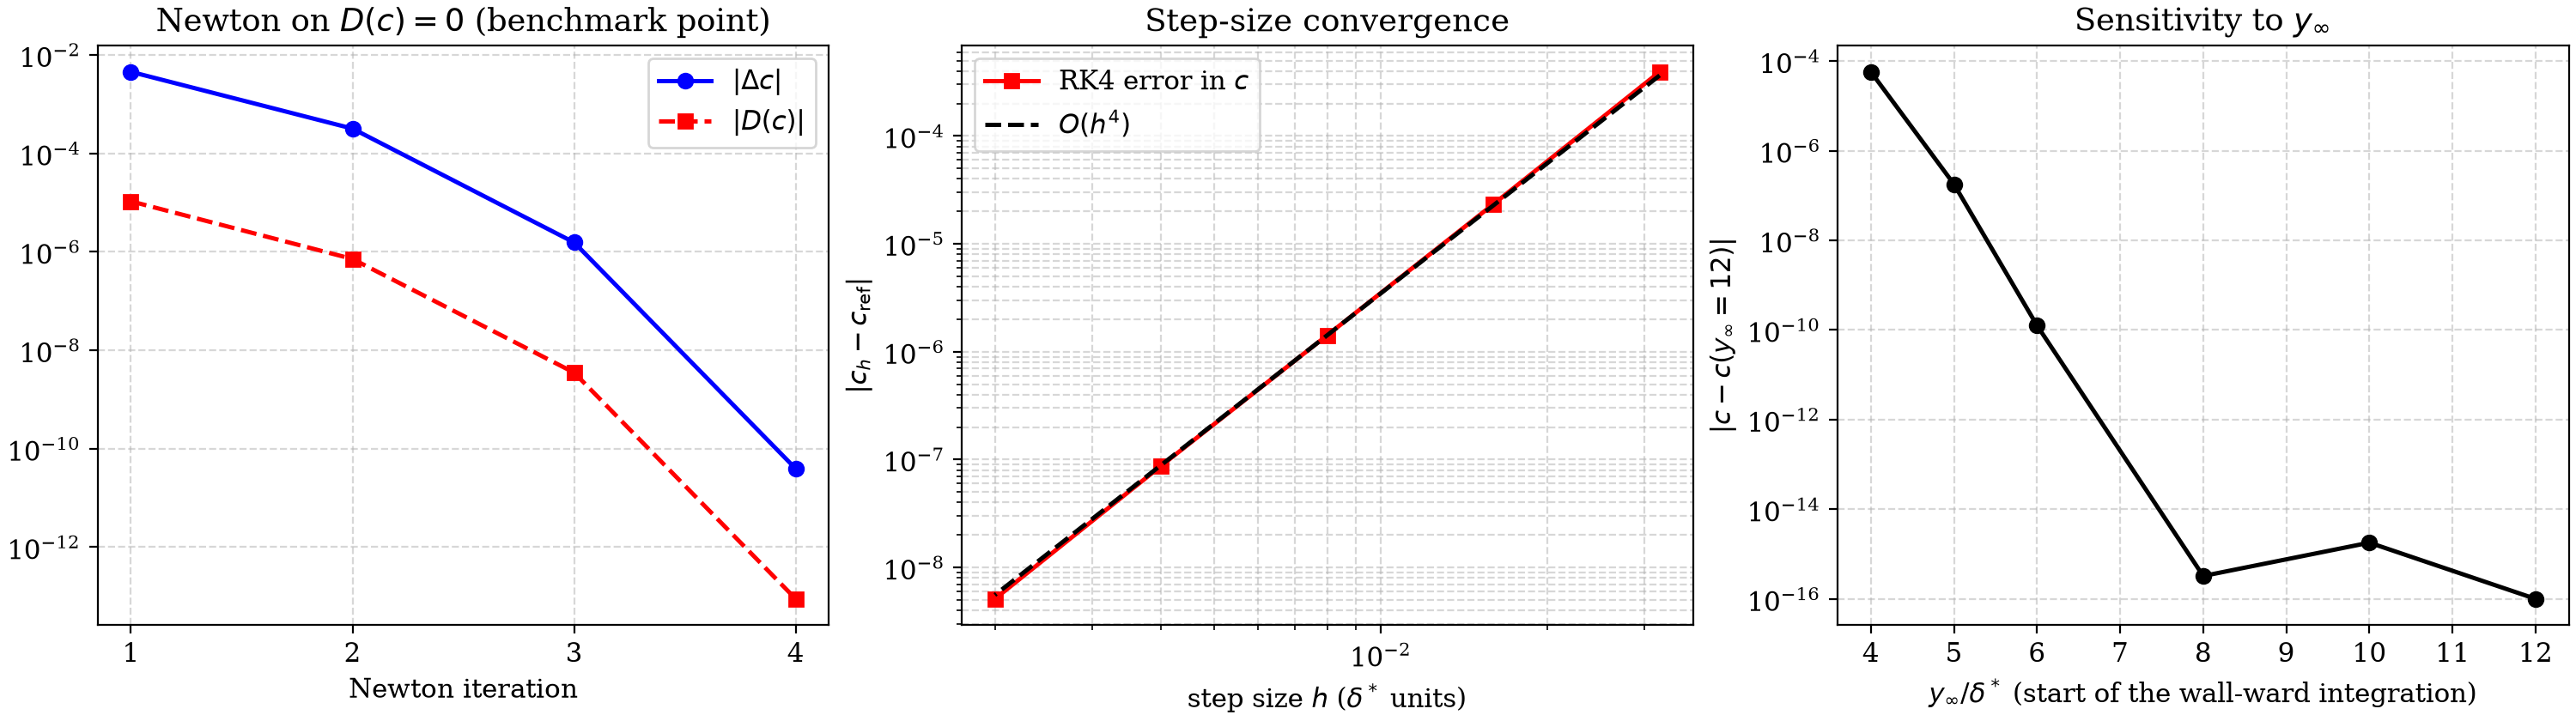
\includegraphics[width=\textwidth]{figures/os_validation.png}
    \caption{Validation at the benchmark point. Left: Newton iterations on $D(c) = 0$. Centre: error in $c$ against RK4 step size, showing 4th-order convergence. Right: sensitivity to the starting height $y_\infty$ of the wall-ward integration.}
    \label{fig:val}
\end{figure}

% ================================================================
\section{Results}
\label{sec:results}
% ================================================================

\subsection{Growth-rate map}

Figure~\ref{fig:cimap} shows $c_i$ for the TS mode over the swept $(Re, \alpha)$ plane, with the refined neutral curve on top. The unstable region ($c_i > 0$) is the familiar tongue that opens to the right of the critical point. The largest growth rates in the swept range, up to $c_i \approx 0.024$, occur for $Re_{\delta^*} \gtrsim 2500$ in the band $\alpha\delta^* \approx 0.1$--$0.2$.

\begin{figure}[h]
    \centering
    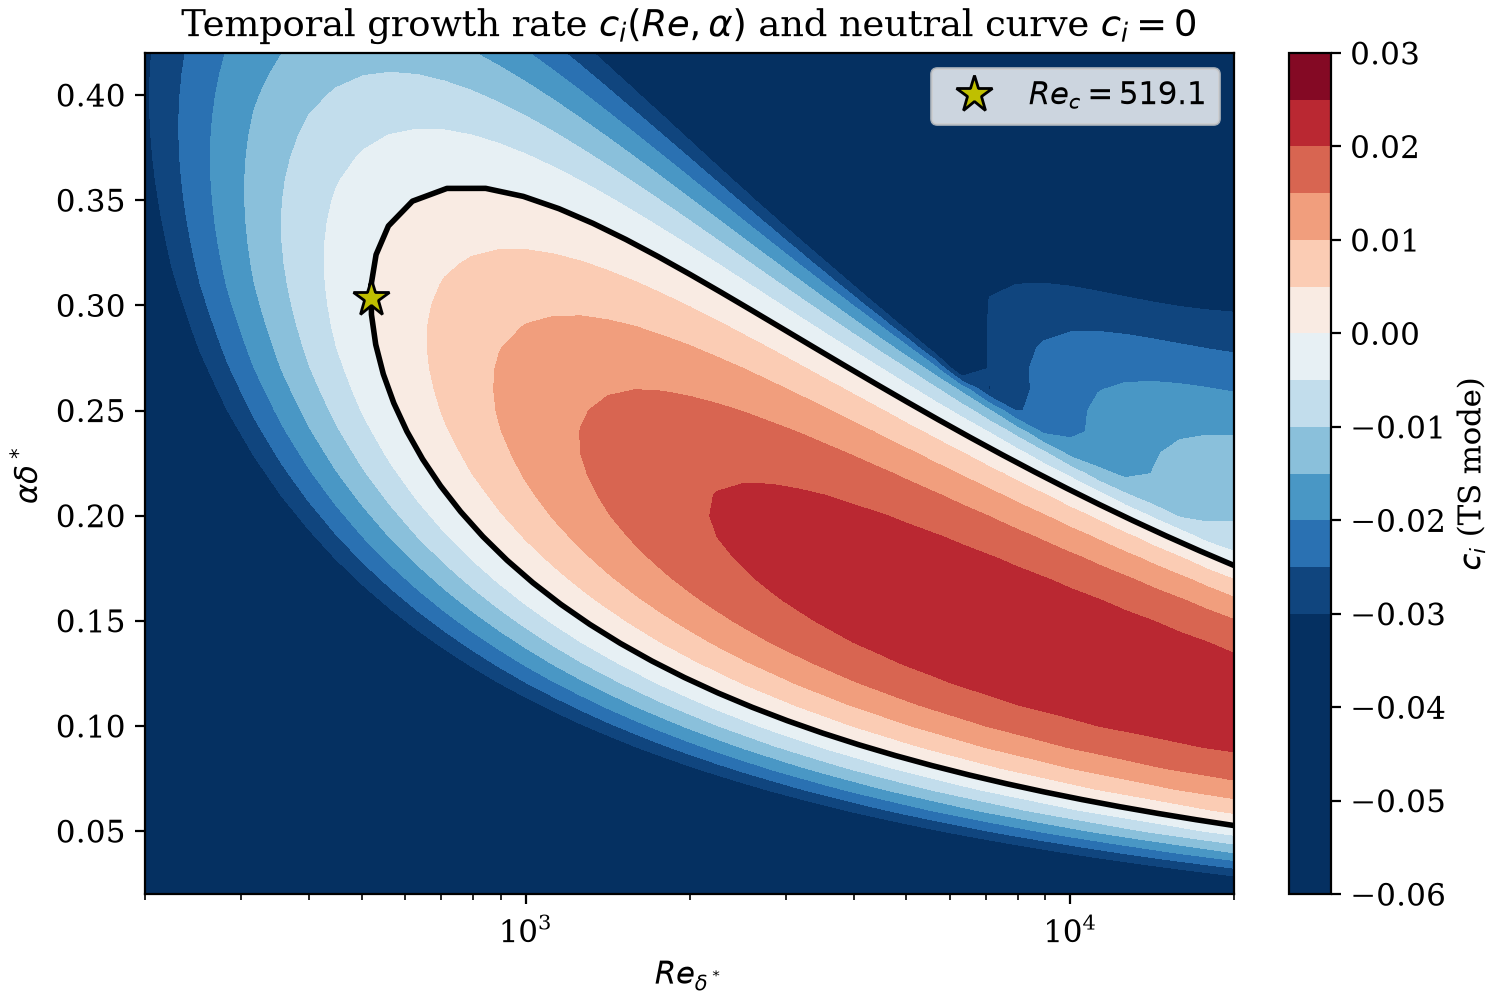
\includegraphics[width=0.85\textwidth]{figures/ci_map.png}
    \caption{Temporal growth rate $c_i(Re, \alpha)$ of the TS mode. The black curve is the refined neutral curve $c_i = 0$ and the star is the critical point.}
    \label{fig:cimap}
\end{figure}

\subsection{Neutral curve}

Figure~\ref{fig:neutral} shows the neutral curve on linear and logarithmic $Re$ axes. The upper branch rises from the nose to a maximum of $\alpha\delta^* \approx 0.355$ near $Re_{\delta^*} \approx 800$, then decreases. The lower branch decreases monotonically. Both branches tend to $\alpha \to 0$ as $Re \to \infty$, which is the expected behaviour for a profile without an inflection point: the band of unstable wavenumbers narrows and the flow becomes stable again in the inviscid limit. Table~\ref{tab:neutral_points} lists neutral wavenumbers and phase speeds at several Reynolds numbers.

\begin{figure}[h]
    \centering
    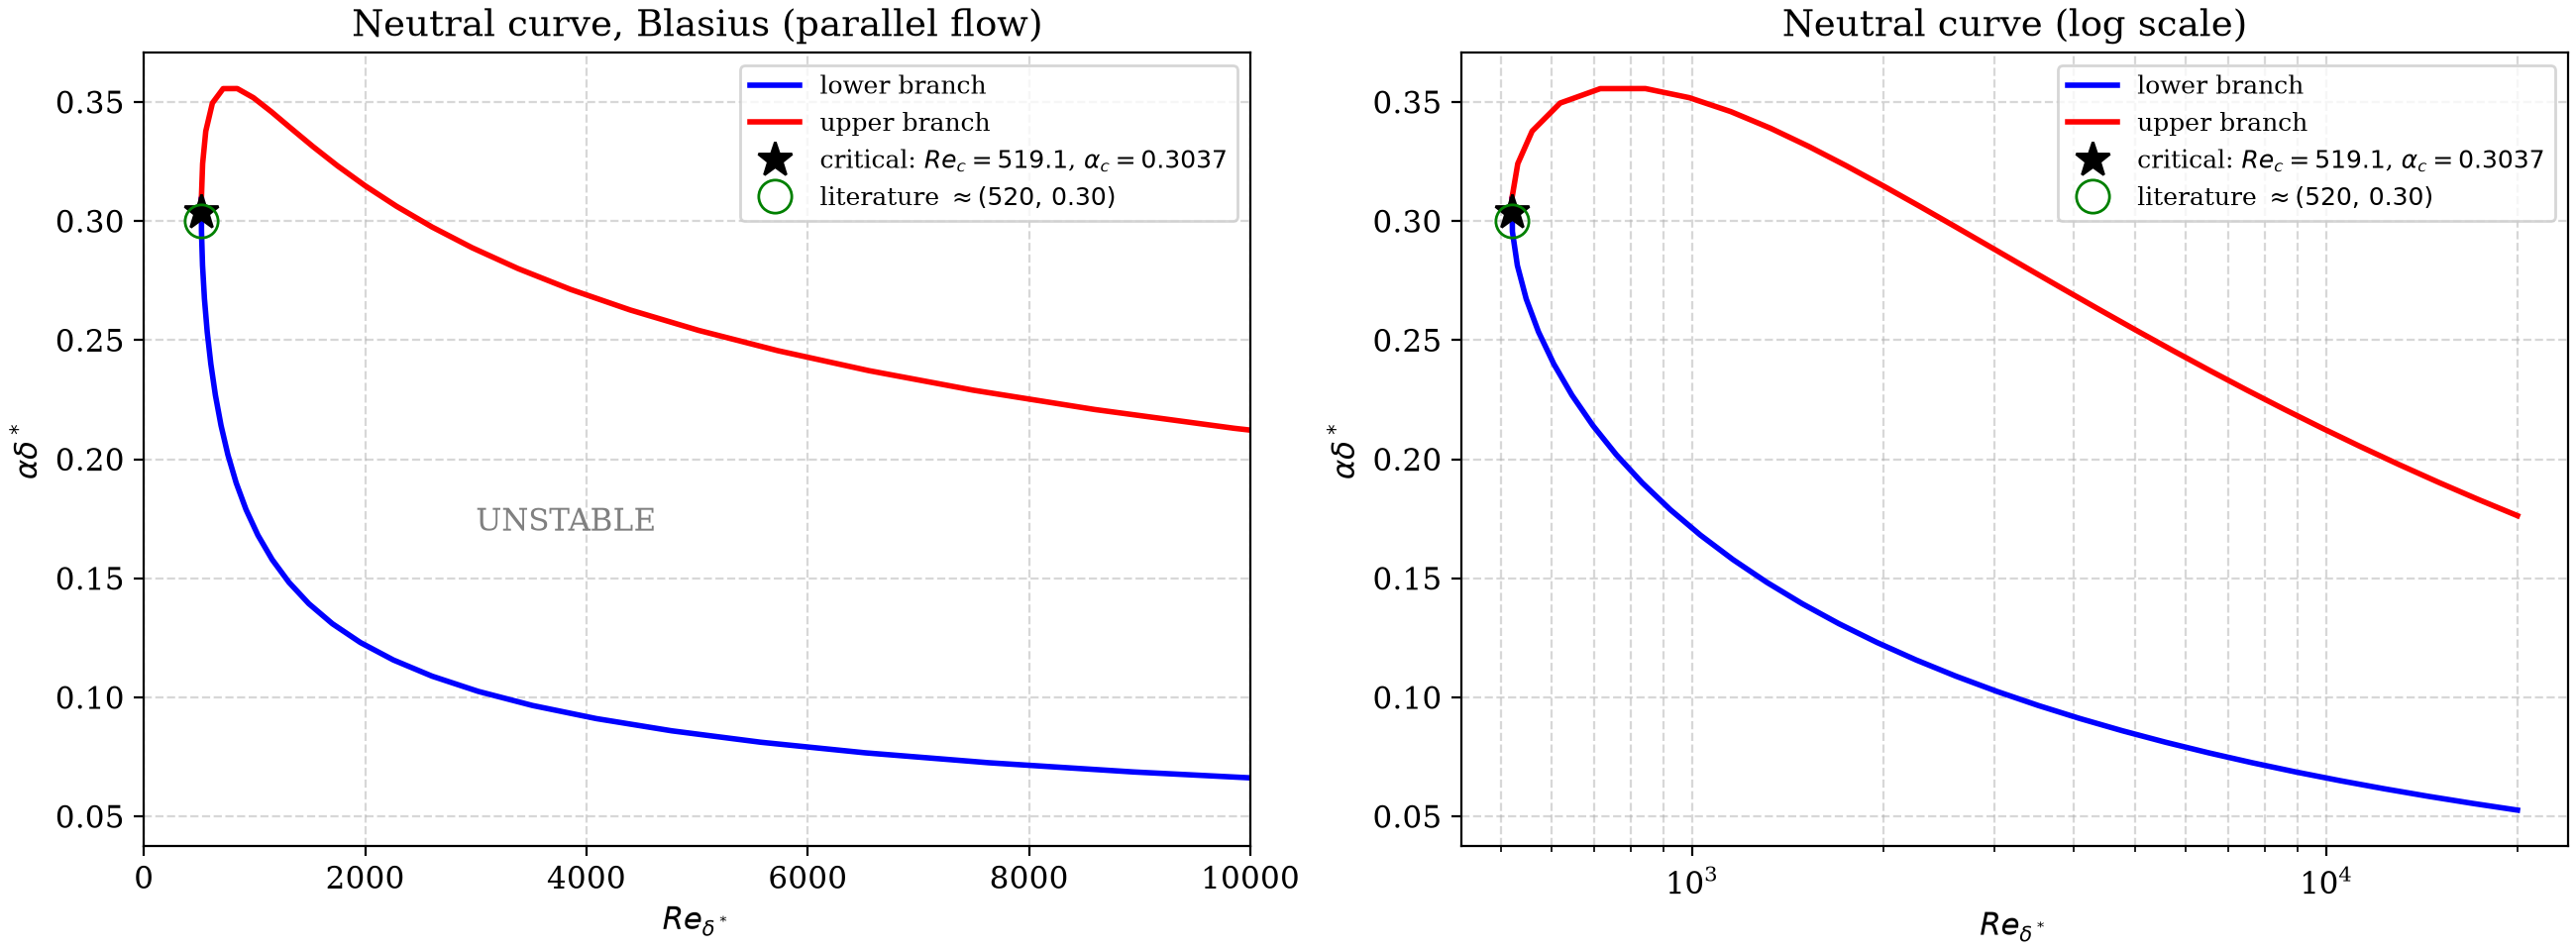
\includegraphics[width=\textwidth]{figures/neutral_curve.png}
    \caption{Neutral stability curve of the Blasius boundary layer (parallel flow), on linear (left) and logarithmic (right) $Re$ axes.}
    \label{fig:neutral}
\end{figure}

\begin{table}[htbp]
  \centering
  \caption{Neutral wavenumbers and phase speeds on the two branches (interpolated from the refined neutral curve).}
  \label{tab:neutral_points}
  \begin{tabular}{lcccc}
    \toprule
    $Re_{\delta^*}$ & $\alpha\delta^*$ (lower) & $c_r$ (lower) & $\alpha\delta^*$ (upper) & $c_r$ (upper) \\
    \midrule
    600 & 0.2420 & 0.3721 & 0.3459 & 0.3979 \\
    1000 & 0.1710 & 0.3223 & 0.3514 & 0.3719 \\
    2000 & 0.1219 & 0.2711 & 0.3148 & 0.3328 \\
    5000 & 0.0845 & 0.2180 & 0.2543 & 0.2846 \\
    10000 & 0.0661 & 0.1852 & 0.2122 & 0.2519 \\
    \bottomrule
  \end{tabular}
\end{table}


\subsection{Critical point and neutral waves}

The minimum Reynolds number on the neutral curve is
\[
    Re_{\delta^*,c} = \osRec, \qquad \alpha_c\delta^* = \osAlphac, \qquad c_r = \osCrc ,
\]
in agreement with the classical parallel-flow result $Re_{\delta^*,c} \approx 520$, $\alpha_c\delta^* \approx 0.30$, $c_r \approx 0.40$~\cite{jordinson1970, schlichting2016}. In terms of distance from the leading edge this is $Re_x = (Re_{\delta^*}/1.7208)^2 \approx 9.1\times10^4$. Neutral waves travel at well below the freestream speed. Figure~\ref{fig:cr} shows their phase speed falling from about $0.40$ at the nose to about $0.19$ on the lower branch at $Re_{\delta^*} = 10^4$, so the critical layer, where $U = c_r$, moves closer to the wall as $Re$ increases.

\begin{figure}[h]
    \centering
    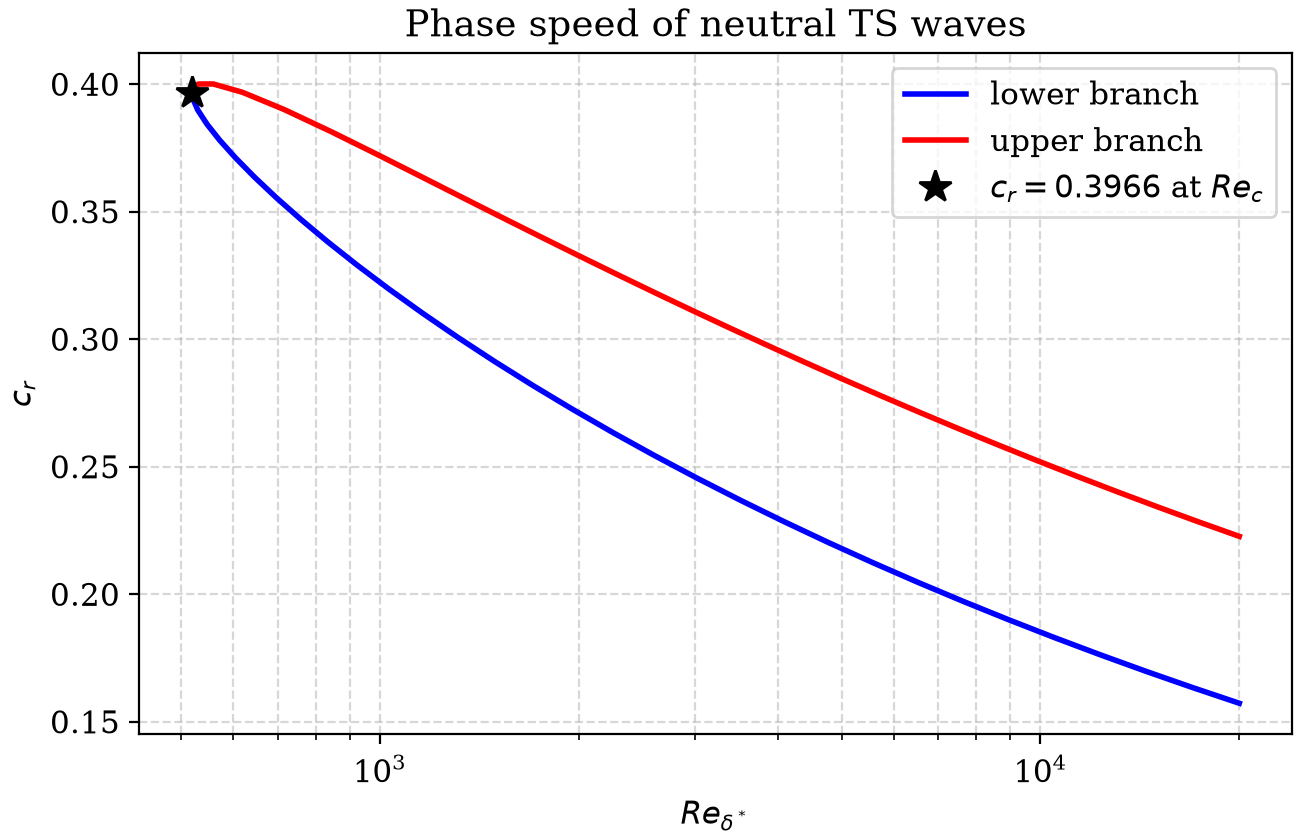
\includegraphics[width=0.65\textwidth]{figures/neutral_phase_speed.png}
    \caption{Phase speed $c_r$ of neutral waves along the lower and upper branches.}
    \label{fig:cr}
\end{figure}

% ================================================================
\section{Discussion and Limitations}
% ================================================================

\begin{itemize}
    \item \textbf{Parallel-flow approximation.} Neglecting the slow growth of the boundary layer gives $Re_{\delta^*,c} \approx 520$. Non-parallel analyses give a somewhat lower critical value, which depends on the disturbance quantity used to define growth. Observed transition occurs much further downstream, at $Re_{\delta^*}$ of order $10^3$, because a TS wave must be amplified by many $e$-folds before nonlinear breakdown.
    \item \textbf{Why shoot from the freestream.} Starting at $y_\infty$ with the exact decaying solutions builds the far-field conditions into the initial data, so only the two wall conditions remain and they collapse to the single complex equation $D = 0$. Shooting from the wall would instead need two unknown wall values and would integrate into the growing freestream solutions.
    \item \textbf{Mode tracking.} The sweep follows the TS eigenvalue by continuation. In the strongly damped corner of the map (large $\alpha$ and $Re \gtrsim 5000$, where $c_i \lesssim -0.03$) the continuation can move onto a different, also damped, eigenvalue, which shows up as a seam in the $c_i$ map. This is far from $c_i = 0$ and does not affect the neutral curve. A global method, such as Chebyshev collocation, would give the whole spectrum and could be used to confirm the mode identity.
    \item \textbf{Cost.} With the vectorised RK4 loop, the Orr--Sommerfeld sweep and refinement take about \osRuntime~s. \texttt{python main.py orr-sommerfeld --quick} runs a coarser grid in about one minute and gives the same critical point to within $0.01$ in $Re$.
\end{itemize}

% ================================================================
\section{Conclusion}
% ================================================================

The Blasius base flow was computed with three independent methods, which agree to $10^{-11}$ and match the classical $f''(0) = 0.332057$ and $\delta^* = 1.7208$. On this profile, shooting the Orr--Sommerfeld equation from the freestream to the wall, with the two decaying solutions carried in compound-matrix form, gives an accurate and robust eigenvalue solver. It reproduces Jordinson's benchmark to $10^{-7}$ and converges at 4th order in the step size. Sweeping the $(Re, \alpha)$ plane and refining the $c_i = 0$ contour gives the Blasius neutral curve, with critical Reynolds number $Re_{\delta^*,c} = \osRec$ at $\alpha_c\delta^* = \osAlphac$ and $c_r = \osCrc$.

\appendix

% ================================================================
\section{Blasius Solver Verification}
\label{app:blasius}
% ================================================================

Figure~\ref{fig:app_bl}(a) shows the error in $f''(0)$ from the scratch RK4 solver against the step size, measured relative to an $h = 0.002$ reference. The observed order rises from about $3.6$ on the coarsest grids to $3.96$, confirming $\mathcal{O}(h^4)$ behaviour. Figure~\ref{fig:app_bl}(b) shows the pointwise difference in $f'(\eta)$ between the methods.

\begin{figure}[h]
    \centering
    \begin{subfigure}[b]{0.48\textwidth}
        \centering
        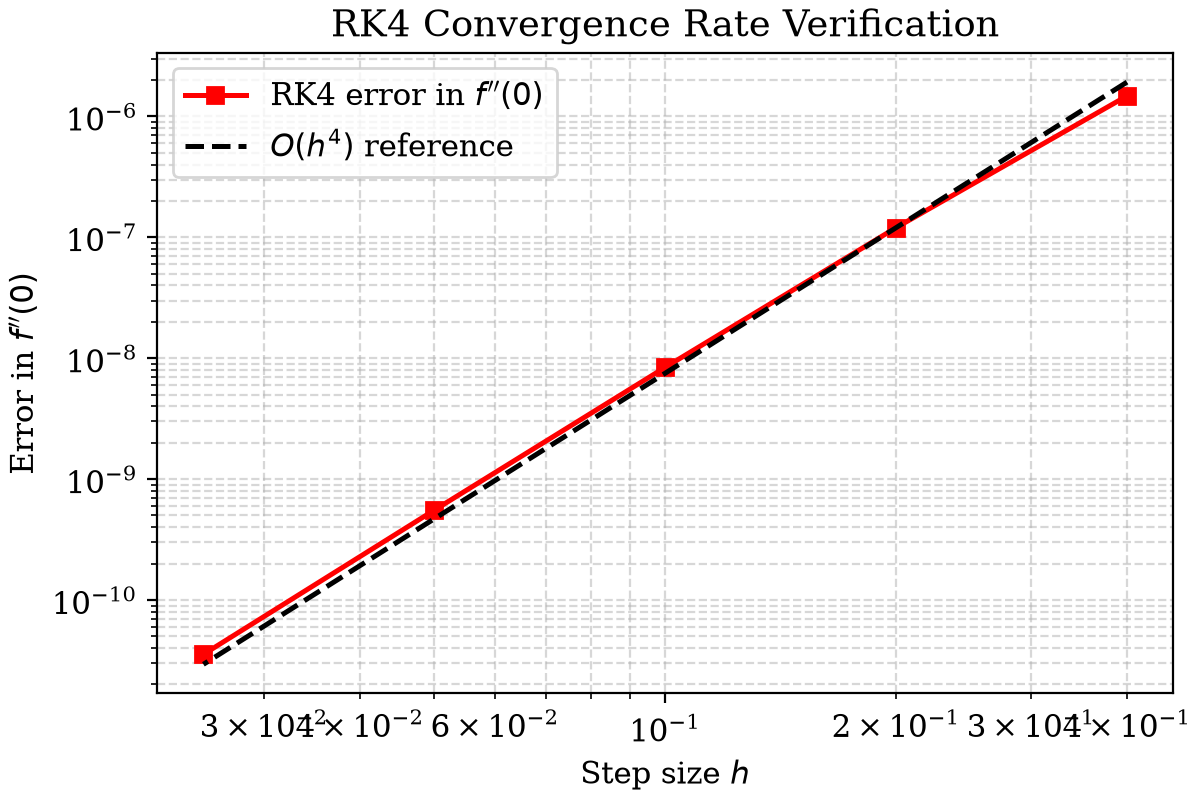
\includegraphics[width=\textwidth]{figures/blasius_rk4_convergence.png}
        \caption{RK4 error in $f''(0)$ against $h$.}
    \end{subfigure}
    \hfill
    \begin{subfigure}[b]{0.48\textwidth}
        \centering
        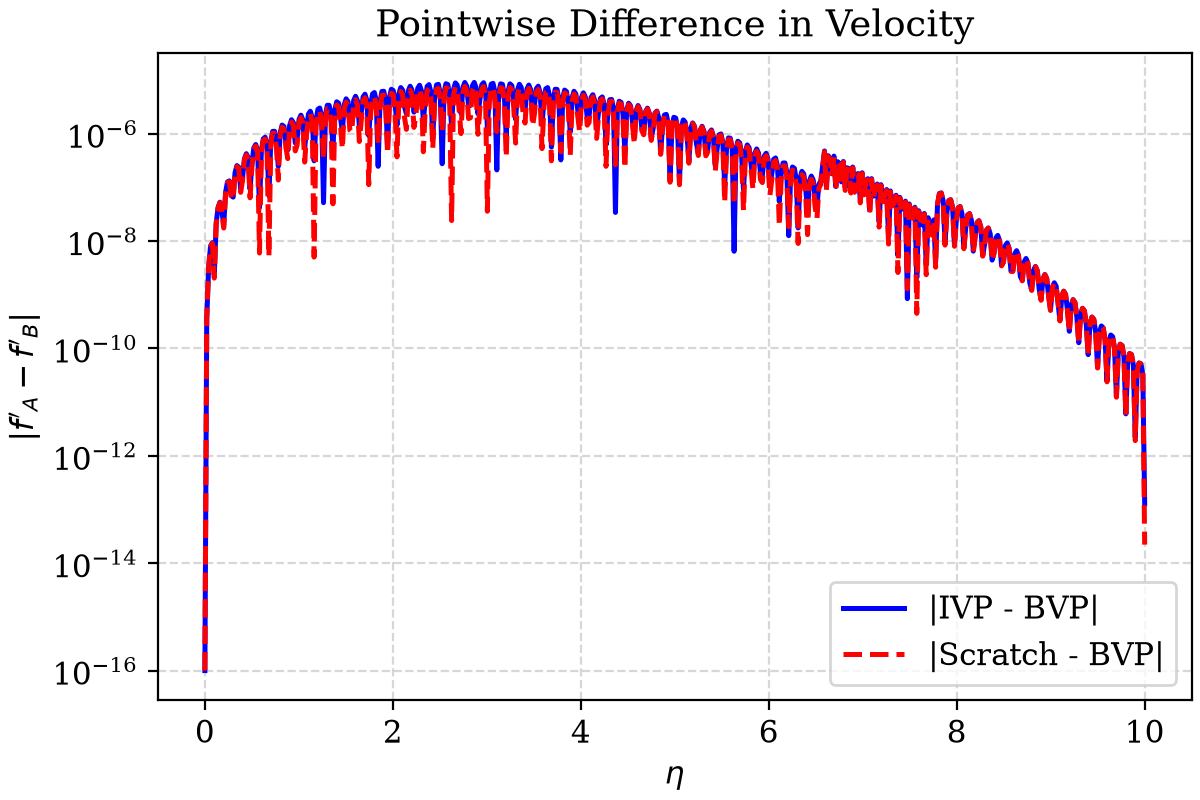
\includegraphics[width=\textwidth]{figures/blasius_method_difference.png}
        \caption{Pointwise $|f'_A - f'_B|$ between methods.}
    \end{subfigure}
    \caption{Verification of the Blasius base-flow solvers.}
    \label{fig:app_bl}
\end{figure}

\begin{thebibliography}{9}

\bibitem{blasius1908}
H.~Blasius, ``Grenzschichten in Flüssigkeiten mit kleiner Reibung,'' \textit{Z. Math. Phys.}, 56:1--37, 1908.

\bibitem{orr1907}
W.~M'F.~Orr, ``The stability or instability of the steady motions of a perfect liquid and of a viscous liquid,'' \textit{Proc. R. Irish Acad. A}, 27:9--138, 1907.

\bibitem{sommerfeld1908}
A.~Sommerfeld, ``Ein Beitrag zur hydrodynamischen Erklärung der turbulenten Flüssigkeitsbewegungen,'' \textit{Proc. 4th Int. Congr. Math.}, Rome, 3:116--124, 1908.

\bibitem{jordinson1970}
R.~Jordinson, ``The flat plate boundary layer. Part 1. Numerical integration of the Orr--Sommerfeld equation,'' \textit{J. Fluid Mech.}, 43(4):801--811, 1970.

\bibitem{ng1979}
B.~S.~Ng and W.~H.~Reid, ``An initial value method for eigenvalue problems using compound matrices,'' \textit{J. Comput. Phys.}, 30:125--136, 1979.

\bibitem{drazin2004}
P.~G.~Drazin and W.~H.~Reid, \textit{Hydrodynamic Stability}, 2nd ed., Cambridge University Press, 2004.

\bibitem{schlichting2016}
H.~Schlichting and K.~Gersten, \textit{Boundary-Layer Theory}, 9th ed., Springer, 2016.

\bibitem{white2006}
F.~M. White, \textit{Viscous Fluid Flow}, 3rd ed., McGraw-Hill, 2006.

\end{thebibliography}

\end{document}
